%======================== PAGE STYLE / LAYOUT ====================%

\documentclass[a4paper,oneside,11pt]{scrartcl}
\usepackage[textwidth=17cm,top=1.5cm,bottom=2.5cm,includehead]{geometry}
\setlength{\textheight}{635pt}
\setlength{\parindent}{0mm} % no paragraph indentation
\setlength{\headsep}{2.5cm}

%============================ PACKAGES ==============================%

\usepackage[T1]{fontenc}        %Umlaute, Sonderzeichen...
\usepackage[utf8]{inputenc}		%Dateicodierung: Unter Linux utf8                                
\usepackage[ngerman]{babel}     %Trennungen, Schriftsatz; Neue deutsche Rechtschreibung
\usepackage[german]{layout}

%========================  STUDENT COMMANDS  ======================%
%% Hier können Sie Ihre eigene LaTeX kommandos hinzufügen. %%

\usepackage{../packages/analysis1_bonn_mathdefs}
\usepackage{../packages/my_header}
\usepackage{../packages/my_assist_packages}
\usepackage{../packages/my_geogebra}
\usepackage{gauss}
\usepackage{pdfpages}


% ===================== Header_Footer ==============================%
%\renewcommand{\headrulewidth}{0pt}
%\renewcommand{\footrulewidth}{0pt}
\usepackage{fancyhdr}
\pagestyle{fancy}
\lhead{\LectureTitle \\ \Semester \\ \LectureType \ (\TutorName)}
\chead{4. Abgabe \\ \today \\}
\rhead{\AuthorOneName \ (\AuthorOneID) \\
\AuthorTwoName \ (\AuthorTwoID) \\ }
%\lfoot{\footnotesize{\AuthorOneName - Matr.: \AuthorOneMatr}}
\cfoot{- \thepage \ -}

%====================================================================%
    
%======================= BEGIN DOCUMENT =============================%
\begin{document}
%\layout

%============ HEADING ===============%
\begin{center}
{\Large{\textbf{Aufgaben für Algorithmische Mathematik 1}}} \\
\end{center}
%====================================%
Die Werte von Bubblesort nähern sich den Polynomen vom Grad $2$ asymptotisch an. Hier sieht man gut, dass beide Polynome in $\cO(n^2)$ liegen.\\
\begin{minipage}[t][4cm][t]{0.49 \textwidth}
\centering
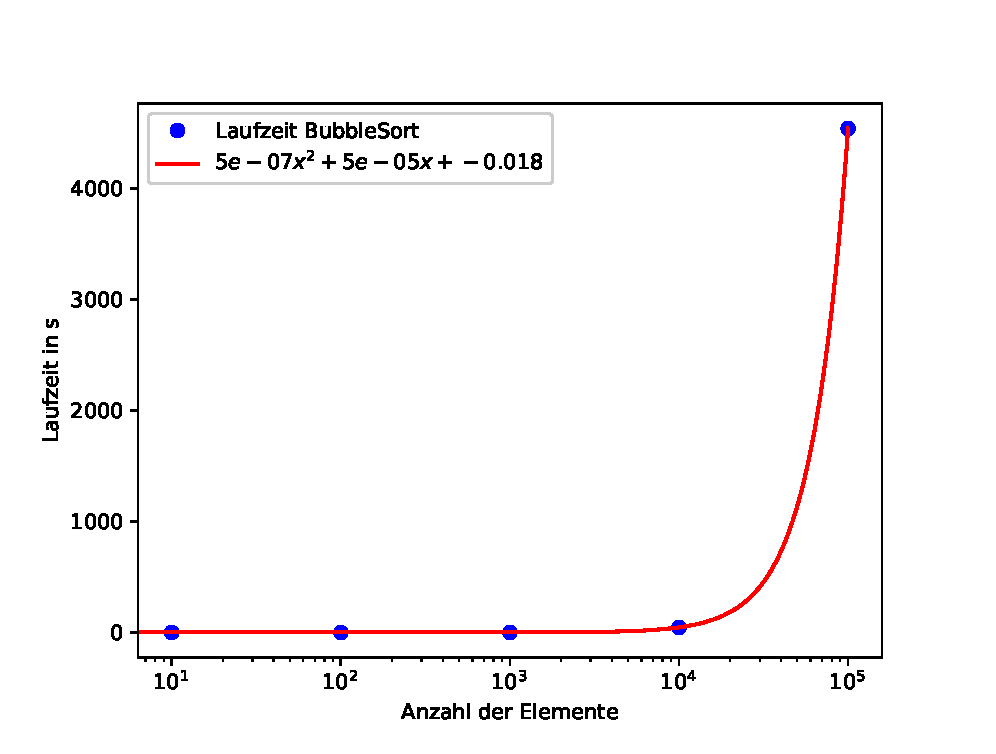
\includegraphics[scale=0.55]{./graphs/laufzeit.eps}
\end{minipage}
\pagebreak
\begin{minipage}[t][4cm][t]{0.49 \textwidth}
\centering
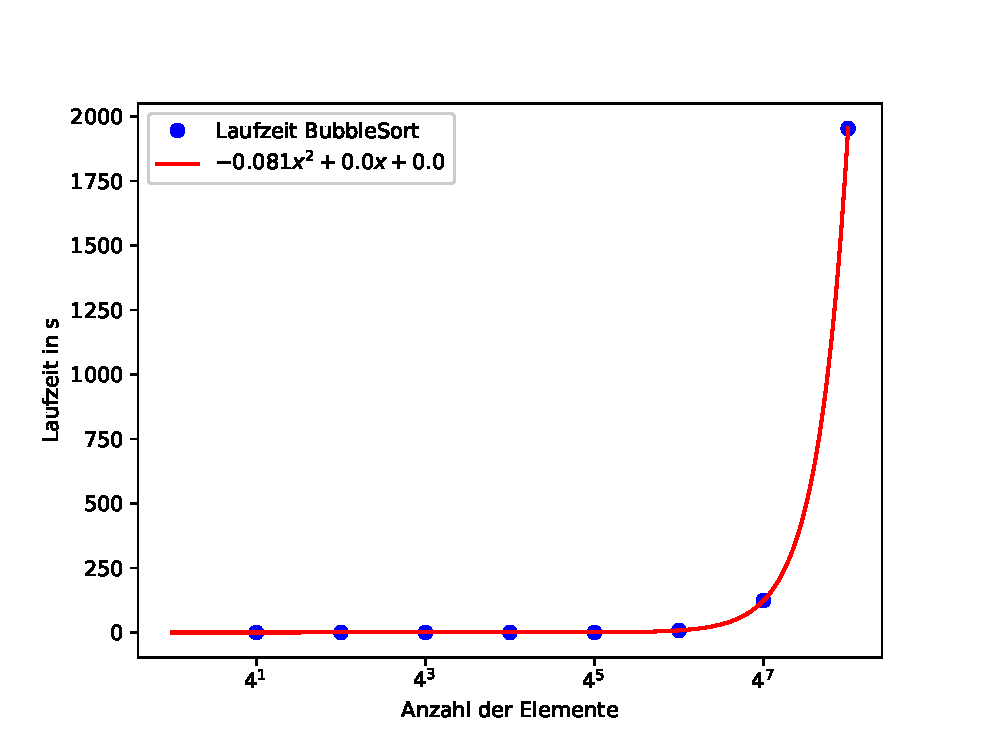
\includegraphics[scale=0.55]{./graphs/laufzeit4.eps}
\end{minipage} \\
Außerdem sieht man auch, dass die Werte ab einem gewissen $n$ immer unter $\cO(n^2)$ liegen werden.
\begin{minipage}[t][4cm][t]{0.49 \textwidth}
\centering
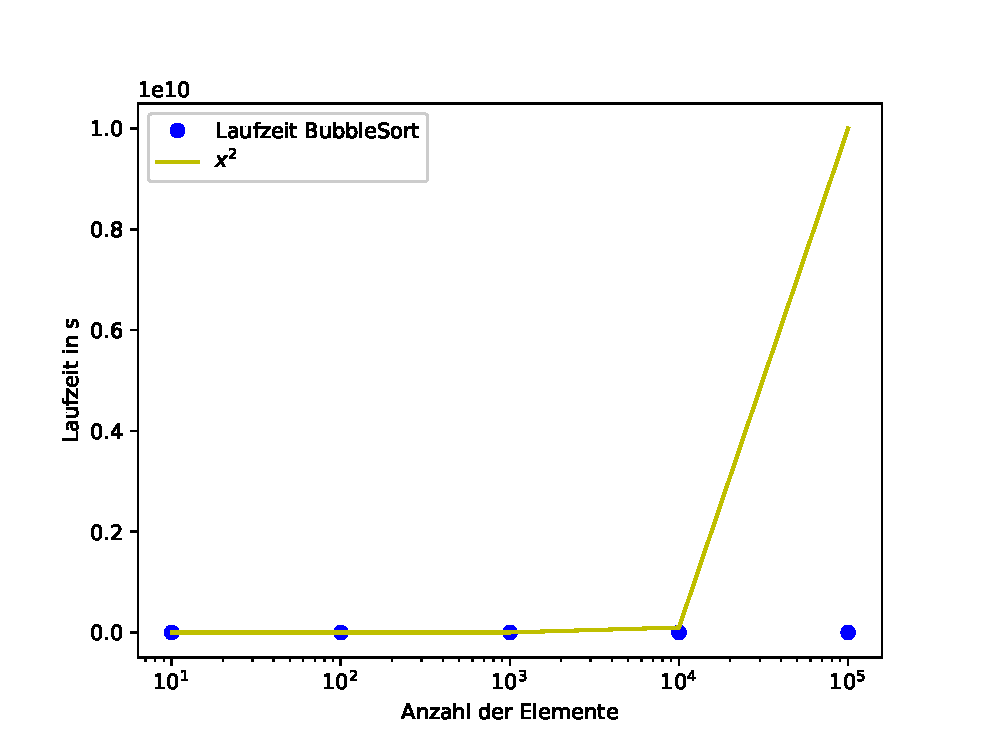
\includegraphics[scale=0.55]{./graphs/laufzeit_1.eps}
\end{minipage}
\end{document}
%===================================== END DOCUMENT ====================================%